\chapter{Variabili aleatorie continue}
Nel Capitolo 4 abbiamo considerato le variabili aleatorie discrete, cioè variabili aleatorie che assumono un numero finito o una infinità numerabile di valori. Tuttavia, vi sono variabili aleatorie il cui insieme dei valori è non numerabile.

\begin{Definition}{Variabile aleatoria continua}{}
    $X$ è una variabile aleatoria continua se esiste una funzione $f:\mathbb{R}\to [0,1]$), tale che per ogni sottoinsieme $B$ di numeri reali ($\forall B\subset\mathbb{R}$):
    \begin{equation*}
        P(X\in B)=\int_Bf(x)dx
    \end{equation*}
    La funzione $f$ è chiamata funzione di densità della variabile aleatoria $X$ (vedi Figura \ref{fig:funzione-di-dentita}) e deve necessariamente valere che $P(-\infty<X<+\infty)=\int^\infty_{-\infty}f(x)dx=1$.
\end{Definition}

\begin{figure}[h]
    \centering
    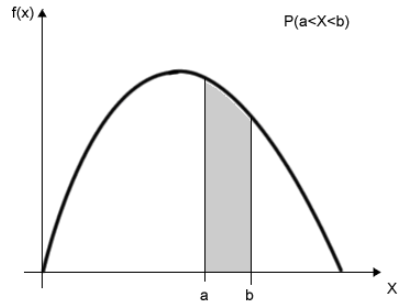
\includegraphics[width=0.5\linewidth]{images/funzione-di-dentita.PNG}
    \caption{Funzione di densità della variabile aleatoria $X$}
    \label{fig:funzione-di-dentita}
\end{figure}

Tutte le affermazioni probabilistiche riguardanti X si possono esprimere in termini di $f$:
\begin{align*}
    P(a\leq X\leq b)=\int^b_af(x)dx\\
    P(X=a)=\int^a_af(x)dx=0
\end{align*}

\begin{Example}{Variabile aleatoria continua}{}
    \textit{Supponiamo che $X$ è una variabile casuale contiua con densità $f(x)$ data da:}
    \begin{equation*}
        f(x)=\begin{cases}
            C(4x-2x^2)\hspace{0.5cm}0<x<2\\0\hspace{0.5cm}\mbox{altrimenti}
        \end{cases}
    \end{equation*}
    \textit{Determinare (a) qual'è il valore di $C$ e (b) $P(X>1)$.}

    \begin{enumerate}[label=(\alph*)]
        \item Dato che $f$ è una densità, si deve avere $\int^\infty_{-\infty}f(x)dx=1$, e pertanto:
        \begin{equation*}
            C\int^2_0(4x-2x^2)dx=1\hspace{1cm}C\left[2x^2-\frac{2x^3}{3}\right]^{2}_{0}=1\hspace{1cm}C=\frac{3}{8}
        \end{equation*}

        \item \begin{equation*}
            P(X>1)=\int^\infty_1f(x)dx=\frac{3}{8}\int^2_1(4x-2x^2)dx=\frac{1}{2}
        \end{equation*}
    \end{enumerate}
\end{Example}

\begin{Example}{Variabile aleatoria continua}{}
    \textit{Il tempo, in ore, che un computer funzioni prima di bloccarsi è una variabile aleatoria continua con densità data da:}
    \begin{equation*}
        f(x)=\begin{cases}
            \lambda e^{-x/100}\hspace{0.5cm}x\geq0\\0\hspace{0.5cm}x<0
        \end{cases}
    \end{equation*}
    \textit{Qual'è la probabilità che (a) il computer funzioni tra le 50 e le 150 ore prima di bloccarsi? (b) il computer funzioni per meno di 100 ore prima di bloccarsi? (c) il computer si rompe esattamente all'istante $t=1.5$?}

    \begin{enumerate}[label=(\alph*)]
        \item Dato che:
        \begin{equation*}
            1=\int^\infty_{-\infty}f(x)dx=\lambda\int^\infty_0e^{-x/100}dx
        \end{equation*}
        si ottiene:
        \begin{equation*}
            1=-\lambda(100)e^{-x/100}\Bigm\lvert^\infty_0=100\lambda\hspace{1cm}\lambda=\frac{1}{100}
        \end{equation*}
        Pertanto la probabilità che un computer funzioni tra le 50 e le 150 ore prima di bloccarsi è data da:
        \begin{equation*}
            P(50<X<150)=\int^{150}_{50}\frac{1}{100}e^{-x/100}dx=e^{-x/100}\Bigm\lvert^{150}_{50}=e^{-1/2}-e^{-3/2}\approx 0.384
        \end{equation*}
        \item Analogamente:
        \begin{equation*}
            P(X<100)=\int^{100}_0\frac{1}{100}e^{-x/100}dx=-e^{-x/100}\Bigm\lvert^{100}_0=1-e^{-1}\approx0.633
        \end{equation*}
        \item
        \begin{equation*}
            P(X=1.5)=\int^{1.5}_{1.5}f(x)dx=0
        \end{equation*}
    \end{enumerate}
\end{Example}

\section{Relazione tra funzione densità e funzione distribuzione}
Se $X$ è una variabile aleatoria continua:
\begin{equation*}
    F(b):=P(X\leq b)=\int^b_{-\infty}f(x)dx\hspace{1cm}f(x)=\frac{d}{dx}F
\end{equation*}
dove $f$ è la densità continua di $X$ e $F$ è la funzione di distribuzione.

\begin{Example}{Relazione tra funzione densità e funzione distribuzione}{}
    \textit{Il numero di persone che entrano in un bar fino al tempo $t$ è una variabile di Poisson $X$ con parametro $\lambda t$. Sia $N$ il primo istante in cui entra una persona nel negozio determinare: (a) la densità discreta di $X$; (b) la funzione di distribuzione di $N$; (c) se $N$ è una variabile aleatoria discreta o continua; (d) la funzione di densità di $N$.}

    \begin{enumerate}[label=(\alph*)]
        \item  $X\sim Poi(\lambda t)$:
        \begin{equation*}
            p(i)=P(X=i)=e^{-\lambda t}\frac{(\lambda t)^i}{i!}
        \end{equation*}
        \item
        \begin{equation*}
            F(b\leq N)=1-P(N>b)=1-(X=0)=\begin{cases}
                1-e^{-\lambda b}\hspace{0.5cm}b\geq0\\0\hspace{1.6cm}b<0
            \end{cases}
        \end{equation*}
        \item $N$ è una variabile aleatoria continua.
        \item
        \begin{equation*}
            f(x)=\frac{d}{dx}F(x)=\begin{cases}
                \frac{d}{dx}(1-e^{-\lambda x})\hspace{0.5cm}x\geq0\\\frac{d}{dx}0=0\hspace{1.3cm}x<0
            \end{cases}=\begin{cases}
                \lambda e^{-\lambda x}\hspace{0.5cm}x\geq0\\0\hspace{1.3cm}x<0
            \end{cases}
        \end{equation*}
    \end{enumerate}
\end{Example}

\section{Valore atteso e varianza di una variabile aleatoria continua}
Se $X$ è una variabile aleatoria continua si definiscono il valore atteso e la varianza di $X$ come:
\begin{gather*}
    E(X)=\int^\infty_{-\infty}xf(x)dx\\
    E(g(x))=\int^\infty_{-\infty}g(x)f(x)dx\\
    E(aX+b)=aE(x)+b\\
    Var(X)=E((X-\mu)^2)=\int^\infty_{-\infty}(x-\mu)^2f(x)dx=E(X^2)-(E(X))^2\\
    Var(aX+b)=a^2Var(X)
\end{gather*}

\begin{Example}{Valore atteso e varianza di una variabile aleatoria continua}{}
    \textit{Un bastoncino di lunghezza 1 è spezzato in un punto $U$ che è distribuito uniformemente su $(0,1)$. Determinare il valore atteso della lunghezza del pezzo di bastoncino che contiene il punto $p,0\leq p\leq 1$.}

    Sia $L_p(U)$ la lunghezza del pezzo di bastoncino, e si osservi che:
    \begin{equation*}
        L_p(U)=\begin{cases}
            1-U\hspace{0.5cm}U<p\\U\hspace{1cm}U>p
        \end{cases}
    \end{equation*}
    Segue che:
    \begin{equation*}
        E(L_p(U))=\int^1_0L_p(u)du=\int^p_0(1-u)du+\int^1_pudu=\frac{1}{2}-\frac{(1-p)^2}{2}+\frac{1}{2}-\frac{p^2}{2}=\frac{1}{2}+p(1-p)
    \end{equation*}
    Dato che $p(1 - p)$ è massimo quando $p =\frac{1}{2}$ si ottiene così che il valore atteso della lunghezza del pezzo di bastoncino che contiene il punto $p$ è massimo quando $p$ è il punto di mezzo del bastoncino originale. 
\end{Example}

Vi sono varie classi importanti di variabili aleatorie che appaiono spesso nelle applicazioni della probabilità; le prossime sezioni sono dedicate al loro studio.

\section{Variabile aleatoria uniforme}
\begin{Definition}{Variabile aleatoria uniforme}{}
    Una variabile aleatoria continua $X$ si dice uniforme (o uniformemente distribuita) se ha funzione di densità:
    \begin{equation*}
        f(x)=\begin{cases}
            1\hspace{0.5cm}0<x<1\\0\hspace{0.5cm}\mbox{altrimenti}
        \end{cases}
    \end{equation*}
    scriviamo $X\sim Unif([0,1])$.

    \textit{Si usa l'uniforme quando gli eventi hanno la stessa probabilità di verificarsi nell'intervallo $(a,b)$.}
\end{Definition}

Da questa formula definisce effettivamente una densità, dato che $f(x)\geq 0$ e $\int^\infty_{-\infty}f(x)dx=\int^1_0dx=1$. Dato che $f(x)> 0$ solo se $x\in (0,1)$, $X$ assume necessariamente almeno un valore in $(0,1)$. Inoltre, essendo $f(x)$ costante per $x\in (0,1)$, $X$ sarà con la stessa probabilità vicino a un qualunque valore di $(0,1)$. Più precisamente si ha, per ogni $0 < a < b < 1$:
\begin{equation*}
    P(a\leq X\leq b)=\int^b_af(x)dx=b-a
\end{equation*}
In altri termini, la probabilità che $X$ stia in un particolare intervallo di $(0,1)$ è uguale all'ampiezza dell'intervallo. In generale, diciamo che $X$ è una variabile aleatoria uniforme sull'intervallo $(\alpha, \beta)$ se la sua densità è data da:
\begin{equation*}
    f(x)=\begin{cases}
        \frac{1}{\beta-\alpha}\hspace{0.5cm}\alpha<x<\beta\\0\hspace{1cm}\mbox{altrimenti}
    \end{cases}
\end{equation*}

Essendo $F(a)=\int^a_{-\infty}f(x)dx$, si ottiene che la funzione di distribuzione di una variabile aleatoria uniforme sull'intervallo $(\alpha, \beta)$ è data da:
\begin{gather*}
    F(a)=\begin{cases}
        0\hspace{1cm}a\leq \alpha\\
        \frac{a-\alpha}{\beta-\alpha}\hspace{0.5cm}\alpha<a<\beta\\
        1\hspace{1cm}a\geq\beta
    \end{cases}\\
    E(X)=\frac{\alpha+\beta}{2}\\
    E(X^2)=\frac{\alpha^2+\alpha\beta+\beta^2}{3}\\
    Var(X)=\frac{(\beta-\alpha)^2}{12}
\end{gather*}

\section{Variabile aleatoria normale}
\begin{Definition}{Variabile aleatoria normale o Gaussiana}{}
    $X$ si dice variabile aleatoria normale (o Gaussiana) con parametri $\mu\in\mathbb{R}$ (media) e $\sigma^2\geq0$ (deviazione standard) se la sua densità è data da:
    \begin{equation*}
        f(x)=\frac{1}{\sqrt{2\pi}\sigma}e^{-\frac{(x-\mu)^2}{2\sigma^2}}
    \end{equation*}
    scriviamo $X\sim N(\mu, \sigma^2)$.

    \textit{Si usa la normale per descrivere fenomeni naturali attorno ad un valore dato $\mu$.}
\end{Definition}
Per provare che $f(x)$ è una densità, dobbiamo mostrare che:
\begin{equation*}
    \frac{1}{\sqrt{2\pi}\sigma}\int^\infty_{-\infty}e^{-\frac{(x-\mu)^2}{2\sigma^2}}dx=1
\end{equation*}

Su una variabile aleatoria normale abbiamo che:
\begin{gather*}
    E(X)=\mu\\
    Var(X)=\sigma^2
\end{gather*}

Dato che $Z=\frac{(X-\mu)}{\sigma}$ è una variabile normale standard ($Z\sim N(0,1)$) se $X$ è normale di parametri $\mu$ e $\sigma^2$, la funzione di distribuzione di $X$ si può scrivere come:
\begin{equation*}
    F(b)=P(Z\leq b)=P\left(\frac{X-\mu}{\sigma}\leq\frac{b-\mu}{\sigma}\right)=\Phi\left(\frac{b-\mu}{\sigma}\right)
\end{equation*}

Tradizionalmente si indica la funzione di distribuzione di una variabile normale standard con $\Phi(b)$. Si pone cioè:
\begin{gather*}
    \Phi(b)=\frac{1}{\sqrt{2\pi}}\int^b_{-\infty}e^{-\frac{t^2}{2}}dt
\end{gather*}

I valori di $\Phi(b)$ per $b$ non negativi sono dati nella Tabella \ref{fig:tabella-var-normale}. Per valori negativi di $b$, $\Phi(b)$ si può ottenere da:
\begin{equation*}
    \Phi(-b)=1-\Phi(b)\hspace{1cm}P(Z>b)=P(Z\leq-b)\hspace{1cm}P(a<Z<b)=\Phi(b)-\Phi(a)
\end{equation*}

\begin{figure}[h]
    \centering
    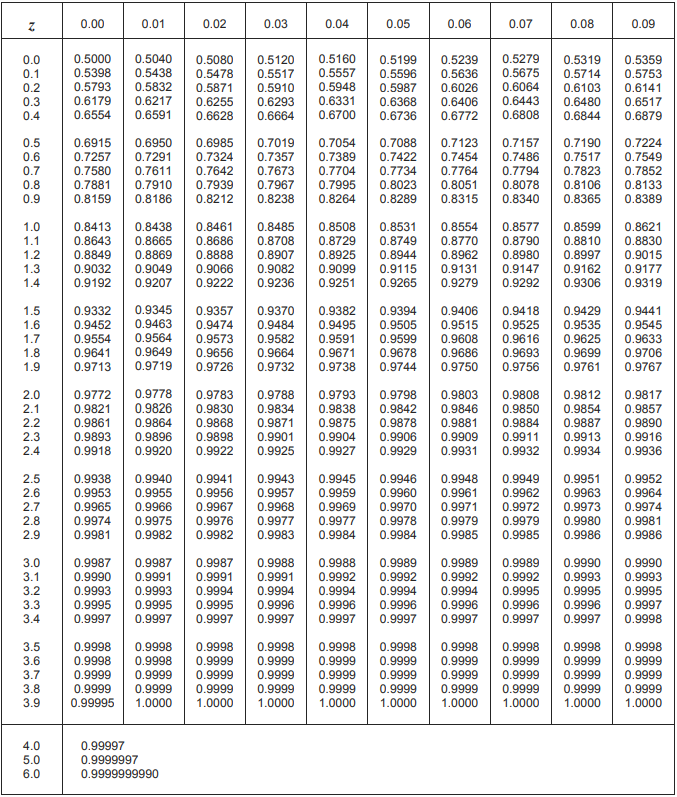
\includegraphics[width=1\linewidth]{images/tabella-var-normale.png}
    \caption{Tabella dei valori di distribuzione normale $\Phi(z)$}
    \label{fig:tabella-var-normale}
\end{figure}

\begin{Example}{Variabile aleatoria normale}{}
    \textit{Sia X una variabile aleatoria normale di parametri $\mu=3$ e $\sigma^2=9$, determinare: (a) $P(2>X>5)$; (b) $P(X>0)$; $P(|X-3|>6)$.}

    \begin{enumerate}[label=(\alph*)]
        \item 
        \begin{align*}
            P(2<X<5)=P\left(\frac{2-3}{3}<\frac{X-3}{3}<\frac{5-3}{3}\right)=P\left(-\frac{1}{3}<Z<\frac{2}{3}\right)=\\\Phi\left(\frac{2}{3}\right)-\Phi\left(-\frac{1}{3}\right)=\Phi\left(\frac{2}{3}\right)-\left[1-\Phi\left(\frac{1}{3}\right)\right]\approx0.3779
        \end{align*}
        \item 
        \begin{align*}
            P(X>0)=P\left(\frac{X-3}{3}>\frac{0-3}{3}\right)=P(Z>-1)=1-\Phi(-1)=\Phi(1)\approx0.8413
        \end{align*}
        \item 
        \begin{align*}
            P(|X-3|>6)=&P(X>9)+P(X<-3)\\=&P\left(\frac{X-3}{3}>\frac{9-3}{3}\right)+P\left(\frac{X-3}{3}<\frac{-3-3}{3}\right)\\=&P(Z>2)+P(Z<-2)=1-\Phi(2)+\Phi(-2)=2[1-\Phi(-2)]\approx 0.0456
        \end{align*}
    \end{enumerate}
\end{Example}

\section{Variabile aleatoria esponenziale}
\begin{Definition}{Variabile aleatoria esponenziale}{}
    Una variabile aleatoria si dice esponenziale (o distribuita esponenzialmente) con parametro $\lambda>0$ se la sua densità è:
    \begin{equation*}
        f(x)=\begin{cases}
            \lambda e^{-\lambda x}\hspace{0.5cm}\mbox{se }x\geq0\\0\hspace{1.2cm}\mbox{se }x<0
        \end{cases}
    \end{equation*}
    scriviamo $X\sim Exp(\lambda)$.

    \textit{Si usa l'esponenziale per il tempo di vita di qualcosa.}
\end{Definition}

$f(x)$ è una densità dato che $\int^\infty_{-\infty}f(x)dx=\int^\infty_0\lambda e^{-\lambda x}dx=\lambda\left[-\frac{1}{\lambda}e^{-\lambda}\right]^\infty_0=\lambda\left[0-\left(-\frac{1}{x}\right)\right]=1$.

La distribuzione $F(b)$ di una variabile aleatoria esponenziale è data da:
\begin{gather*}
    F(b)=P(X\leq b)=\int^b_0\lambda e^{-\lambda x}dx=-e^{-\lambda x}\Bigm\lvert^b_0=1-e^{-\lambda b}\\
    F(b)=\begin{cases}
        1-e^{-\lambda b}\hspace{0.5cm}\mbox{se }b\geq0\\
        0\hspace{1.6cm}\mbox{se }b<0
    \end{cases}\\
    E(X)=\int^\infty_0x\lambda e^{-\lambda x}dx=-xe^{-\lambda x}\Bigm\lvert^\infty_0+\int^\infty_0e^{-\lambda x}dx=0-\frac{e^{-\lambda x}}{\lambda}\Bigm\lvert^\infty_0=\frac{1}{\lambda}\\
    E(X^2)=\int^\infty_0x^2\lambda e^{-\lambda x}dx=-x^2e^{-\lambda x}\Bigm\lvert^\infty_0+\int^\infty_02xe^{-\lambda x}dx=0+\frac{2}{\lambda}E(X)=\frac{2}{\lambda^2}\\
    Var(X)=\frac{2}{\lambda^2}-\left(\frac{1}{\lambda}\right)^2=\frac{1}{\lambda^2}\\
    P(X>b+a|X>b)=P(X>a)
\end{gather*}

\begin{Example}{Variabile aleatoria esponenziale}{}
    \textit{Supponiamo che la lunghezza di una telefonata in minuti sia una variabile aleatoria esponenziale di parametro $\lambda=\frac{1}{10}$ . Se qualcuno arriva immediatamente prima di voi alla cabina telefonica, determinare la probabilità di dover aspettare (a) più di 10 minuti; (b) tra 10 e 20 minuti.}

    Sia $X$ la lunghezza della telefonata fatta dalla persona che occupa la cabina, le probabilità cercate valgono:
    \begin{enumerate}[label=(\alph*)]
        \item
        \begin{equation*}
            P(X>10)=1-F(10)=e^{-1}\approx 0.368
        \end{equation*}
        \item
        \begin{equation*}
            P(10<X<20)=F(20)-F(10)=e^{-1}-e^{-2}\approx 0.233
        \end{equation*}
    \end{enumerate}
\end{Example}
